\section{Contiki-ng}
\label{sec:contikiNG}

Contiki es un sistema operativo diseñado específicamente para dispositivos de baja capacidad, como sensores. Fue desarrollado por Adam Dunkels en colaboración con Bjorn Gronvall y Thiemo Voigt en 2002. A lo largo de los años, el proyecto Contiki ha crecido enormemente y ha involucrado a numerosas empresas y cientos de colaboradores en su repositorio de GitHub\footnote{\url{https://github.com/contiki-os/contiki}}. El objetivo principal de Contiki era proporcionar a los nodos de las redes de sensores inalámbricos (WSN) un sistema operativo liviano capaz de cargar y descargar servicios de forma dinámica \cite{1367266}.\\
\\
El kernel de Contiki se basa en un modelo orientado a eventos y admite multitarea con prelación. Está escrito en lenguaje C y ha sido portado a diversas arquitecturas de microcontroladores, como el MSP430 de Texas Instruments y sus variantes.\\
\\
En un sistema que ejecuta Contiki, se divide en dos partes claramente diferenciadas del firmware, como se muestra en la Figura \ref{fig:contikiParts}: el núcleo (\textit{core}) y los programas o servicios cargados. Esta partición se realiza durante la etapa de compilación y es independiente del objetivo (target) donde se desplegará el sistema. El núcleo (\textit{core}) incluye el propio kernel, un conjunto de servicios base (como temporizadores y controladores), bibliotecas, controladores y el stack de comunicación. Los programas o servicios cargados se mapean en memoria mediante el cargador del kernel durante el tiempo de ejecución.\\


% Foto 
\begin{figure}[ht]
    \centering
    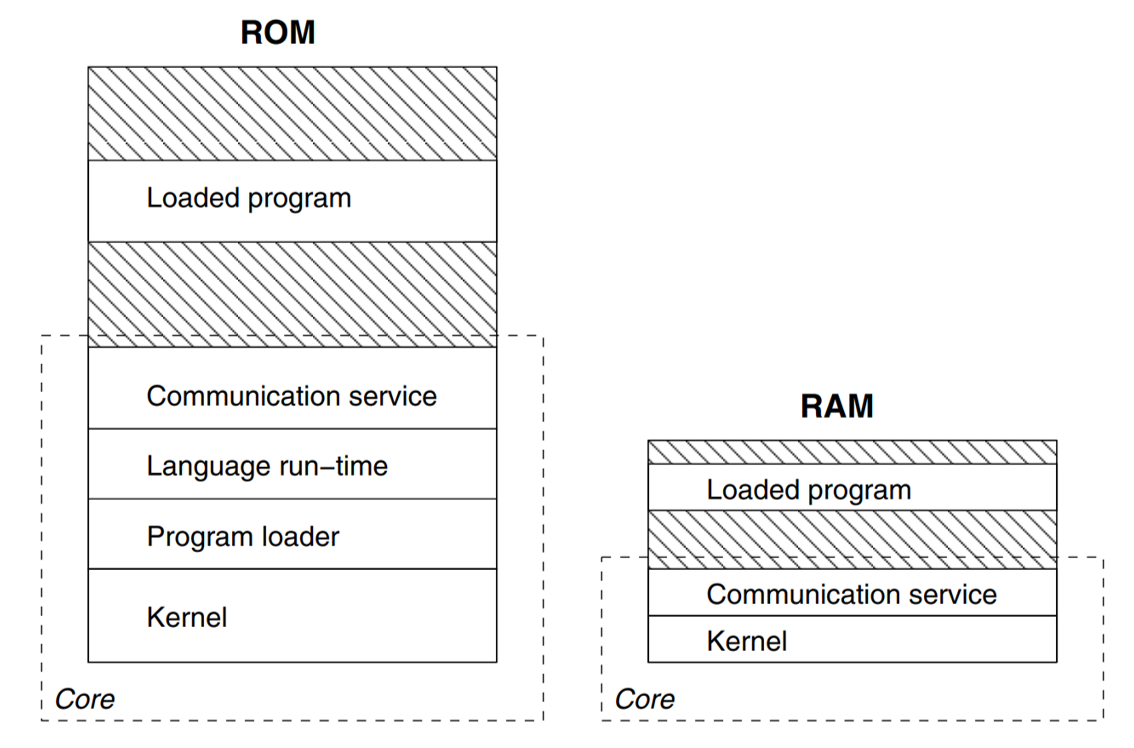
\includegraphics[width=0.8\textwidth]{archivos/img/teoria/contiki.png}
    \caption{Gestión de la memoria en un sistema con Contiki OS \cite{1367266}}
    \label{fig:contikiParts}
\end{figure}


En los últimos años ha surgido un nuevo proyecto llamado \textbf{Contiki-ng}\footnote{\url{https://github.com/contiki-ng/contiki-ng}}, el cual es un fork del sistema operativo Contiki. Este proyecto ha ganado popularidad y ha superado a su predecesor con el eslogan ``Contiki-NG: El sistema operativo para dispositivos IoT de próxima generación". Actualmente, toda la comunidad de Contiki se está centrando en este nuevo proyecto, el cual proporciona un stack de comunicación más compatible con las especificaciones RFC, ofrece soporte para protocolos como IPv6/6LoWPAN y 6TiSCH, y se está volviendo cada vez más popular por su capacidad de brindar soporte a microcontroladores con arquitectura ARM \cite{kurniawan2018practical}.

\subsection{Simulador Cooja}

El flujo de trabajo con Contiki o Contiki-ng varía dependiendo de si se trabaja con hardware real o si se realiza una simulación de los programas desarrollados. En el caso de trabajar con hardware real, el proceso consiste en compilar el sistema operativo y los programas específicos utilizando el objetivo (target) correspondiente, lo que generará un archivo binario que se puede cargar en la memoria del hardware.\\
\\
Por otro lado, si se opta por la simulación, se utilizará el simulador llamado Cooja\footnote{\url{https://github.com/contiki-ng/cooja/tree/master}}. Cooja es un simulador escrito en Java que permite \textbf{simular} una serie de nodos \gls{iot}. Al simular, es posible observar el comportamiento del programa desarrollado en diferentes plataformas. El proceso de compilación del núcleo (core) de Contiki y los programas desarrollados está integrado en el propio simulador, lo que facilita al usuario la compilación de sus programas para diferentes tipos de nodos. Cada simulación se puede guardar en un archivo con extensión \texttt{*.csc}, que almacena todos los datos de la simulación, como la semilla (\textit{seed}), las posiciones y los tipos de nodos, utilizando una estructura XML.\\
\\
De esta manera, tanto si se trabaja con hardware real como si se realiza una simulación, Contiki y Contiki-ng ofrecen herramientas y entornos integrados que permiten desarrollar y probar programas para sistemas embebidos y dispositivos \gls{iot}. A continuación, en la Figura \ref{fig:cooja}, se indica la interfaz gráfica del simulador.

\begin{figure}[ht]
    \centering
    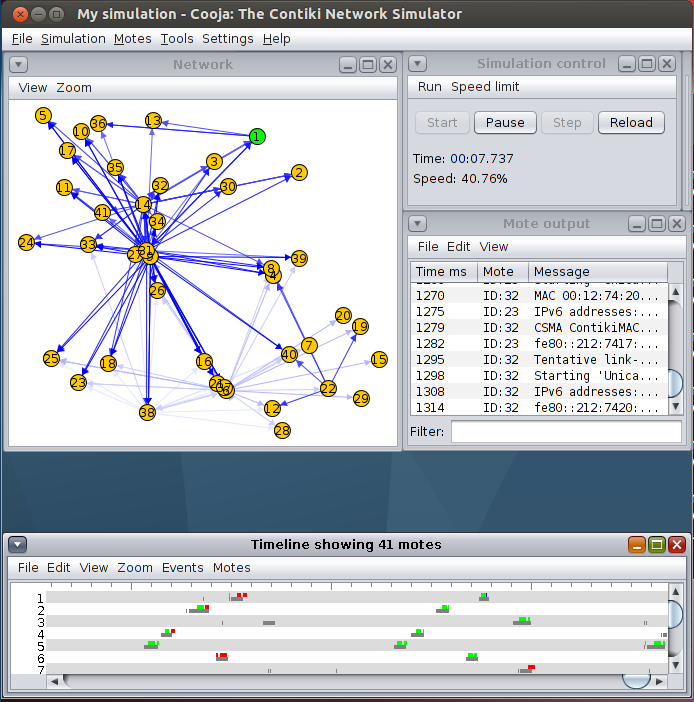
\includegraphics[width=0.6\textwidth]{archivos/img/teoria/cooja.png}
    \caption{Interfaz gráfica del simulador Cooja \cite{cooja1}}
    \label{fig:cooja}
\end{figure}

